\clearpage
\section{\textbf{Appendix}}

\subsection{AMEN Model Convergence}

MCMC chain analysis for AMEN model presented in paper.  

\begin{figure}[ht]
	\centering
	\begin{tabular}{cc}
	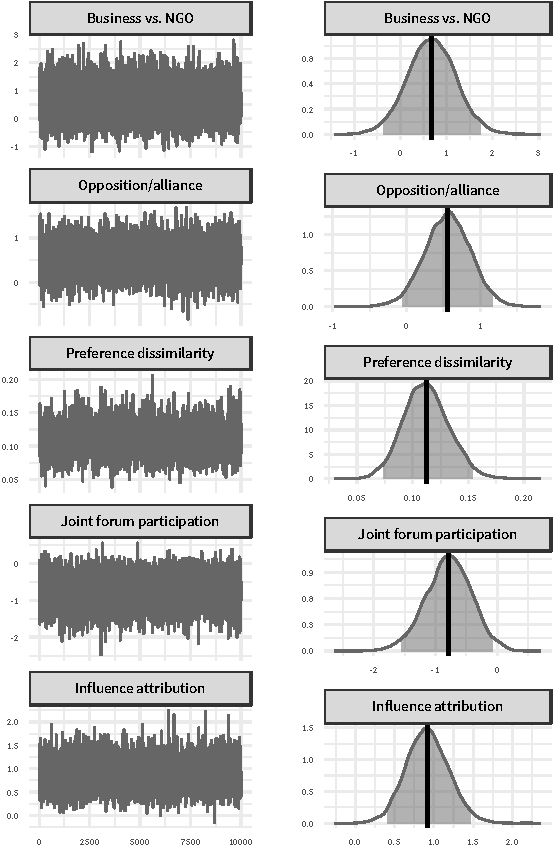
\includegraphics[width=.45\textwidth]{ameConv1_SR2} &
	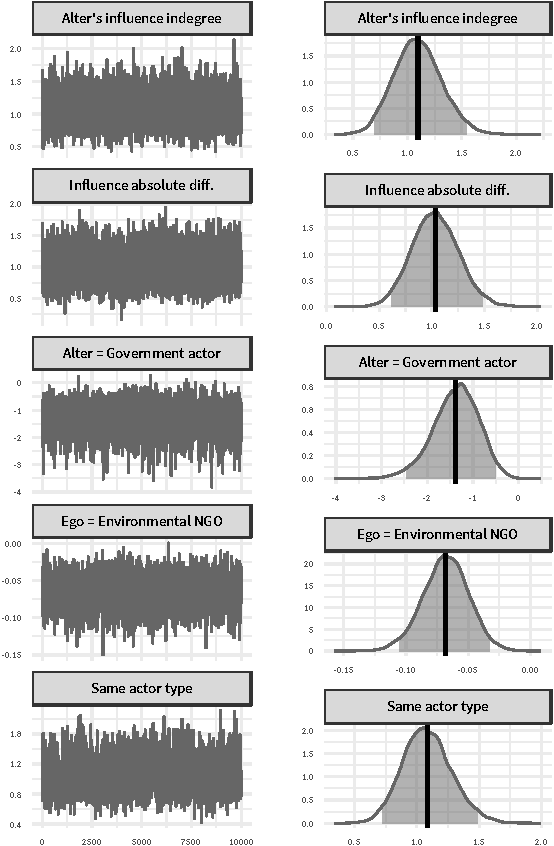
\includegraphics[width=.45\textwidth]{ameConv2_SR2}
	\end{tabular}
	\caption{MCMC chain for AMEN model presented in paper. In this model, we utilize the SRM to account for first and second-order dependence. To account for third order dependencies we use the latent factor approach discussed earlier with $K=2$.}
	\label{fig:ameConv}
\end{figure}
\FloatBarrier
\newpage

\subsection{Comparison of \pkg{amen} \& \pkg{latentnet} $\mathcal{R}$ Packages}

Here we provide a comparison of the AMEN model we presented in the paper with a variety of parameterizations from the \pkg{latentnet} package. 

% latex table generated in R 3.3.1 by xtable 1.8-2 package
% Sun Aug 21 03:38:39 2016
\begin{table}[ht]
\centering
\begingroup\tiny
\begin{tabular}{lccccc}
   & LSM & LSM (Bilinear) & LSM (SR) & LSM (Bilinear + SR) & AME \\ 
  \hline
\hline
Intercept/Edges & 0.94$^{\ast}$ & -2.66$^{\ast}$ & 0.60 & -2.50$^{\ast}$ & -3.39$^{\ast}$ \\ 
   & [0.09; 1.82] & [-3.53; -1.87] & [-1.10; 2.37] & [-4.14; -0.88] & [-4.38; -2.50] \\ 
  \textbf{Conflicting policy preferences} &  &  &  &  &  \\ 
  $\;\;\;\;$ Business vs. NGO & -1.37$^{\ast}$ & -2.64$^{\ast}$ & -3.07$^{\ast}$ & -2.87$^{\ast}$ & -1.37$^{\ast}$ \\ 
   & [-2.42; -0.41] & [-4.61; -0.96] & [-4.77; -1.56] & [-4.63; -1.29] & [-2.44; -0.47] \\ 
  $\;\;\;\;$ Opposition/alliance & 0.00 & 0.04 & 0.31 & 0.24 & 1.08$^{\ast}$ \\ 
   & [-0.40; 0.39] & [-0.44; 0.54] & [-0.24; 0.86] & [-0.36; 0.82] & [0.72; 1.47] \\ 
  $\;\;\;\;$ Preference dissimilarity & -1.76$^{\ast}$ & -2.00$^{\ast}$ & -1.88$^{\ast}$ & -2.20$^{\ast}$ & -0.79$^{\ast}$ \\ 
   & [-2.62; -0.90] & [-3.01; -1.03] & [-3.07; -0.68] & [-3.46; -0.96] & [-1.55; -0.08] \\ 
  \textbf{Transaction costs} &  &  &  &  &  \\ 
  $\;\;\;\;$ Joint forum participation & 1.51$^{\ast}$ & 1.24$^{\ast}$ & 1.56$^{\ast}$ & 1.62$^{\ast}$ & 0.92$^{\ast}$ \\ 
   & [0.86; 2.17] & [0.53; 1.93] & [0.69; 2.41] & [0.70; 2.52] & [0.40; 1.47] \\ 
  \textbf{Influence} &  &  &  &  &  \\ 
  $\;\;\;\;$ Influence attribution & 0.08 & -0.08 & 0.30 & 0.28 & 1.09$^{\ast}$ \\ 
   & [-0.40; 0.55] & [-0.62; 0.46] & [-0.37; 0.96] & [-0.42; 0.97] & [0.69; 1.53] \\ 
  $\;\;\;\;$ Alter's influence indegree & 0.01 & -0.05$^{\ast}$ & 0.06 & 0.05 & 0.11$^{\ast}$ \\ 
   & [-0.03; 0.04] & [-0.09; -0.01] & [-0.03; 0.14] & [-0.04; 0.13] & [0.07; 0.15] \\ 
  $\;\;\;\;$ Influence absolute diff. & 0.04 & 0.02 & -0.08$^{\ast}$ & -0.08$^{\ast}$ & -0.07$^{\ast}$ \\ 
   & [-0.01; 0.09] & [-0.03; 0.07] & [-0.14; -0.02] & [-0.14; -0.02] & [-0.11; -0.03] \\ 
  $\;\;\;\;$ Alter = Government actor & -0.46 & -0.80 & -0.11 & -0.20 & 0.55 \\ 
   & [-1.08; 0.14] & [-1.67; 0.04] & [-1.91; 1.76] & [-2.14; 1.74] & [-0.07; 1.15] \\ 
  \textbf{Functional requirements} &  &  &  &  &  \\ 
  $\;\;\;\;$ Ego = Environmental NGO & -0.60 & -1.90$^{\ast}$ & -1.69 & -1.84 & 0.67 \\ 
   & [-1.32; 0.09] & [-3.10; -0.86] & [-3.74; 0.23] & [-4.02; 0.11] & [-0.38; 1.71] \\ 
  $\;\;\;\;$ Same actor type & 1.17$^{\ast}$ & 1.40$^{\ast}$ & 1.82$^{\ast}$ & 1.90$^{\ast}$ & 1.04$^{\ast}$ \\ 
   & [0.63; 1.71] & [0.85; 1.95] & [1.10; 2.54] & [1.19; 2.62] & [0.63; 1.50] \\ 
   \hline
\hline
\end{tabular}
\endgroup
\caption{* p $<$ 0.05. 95\% posterior credible intervals are provided in brackets.} 
\label{tab:regTable_latSpace}
\end{table}


\begin{figure}[ht]
	\centering
	\begin{tabular}{cc}
	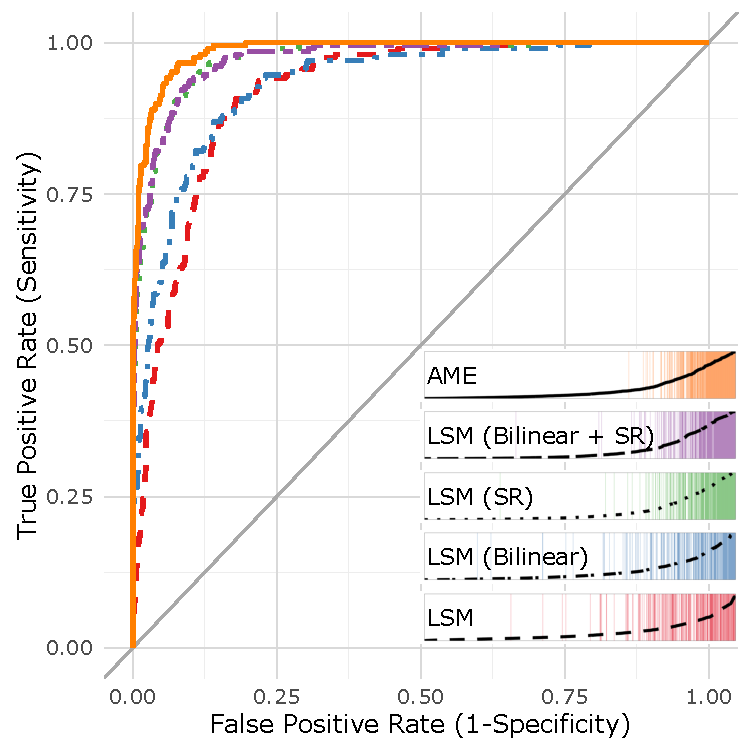
\includegraphics[width=.5\textwidth]{roc_latSpace} & 
	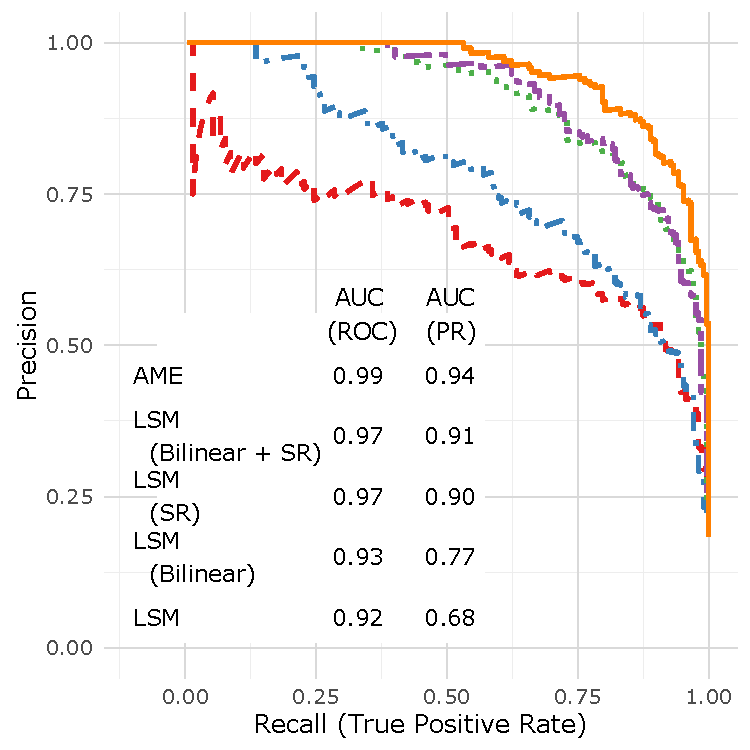
\includegraphics[width=.5\textwidth]{rocPr_latSpace}
	\end{tabular}
	\caption{ROC and separation plots}
	\label{fig:roc_latentSpace}
\end{figure}

\begin{figure}[ht]
	\centering
	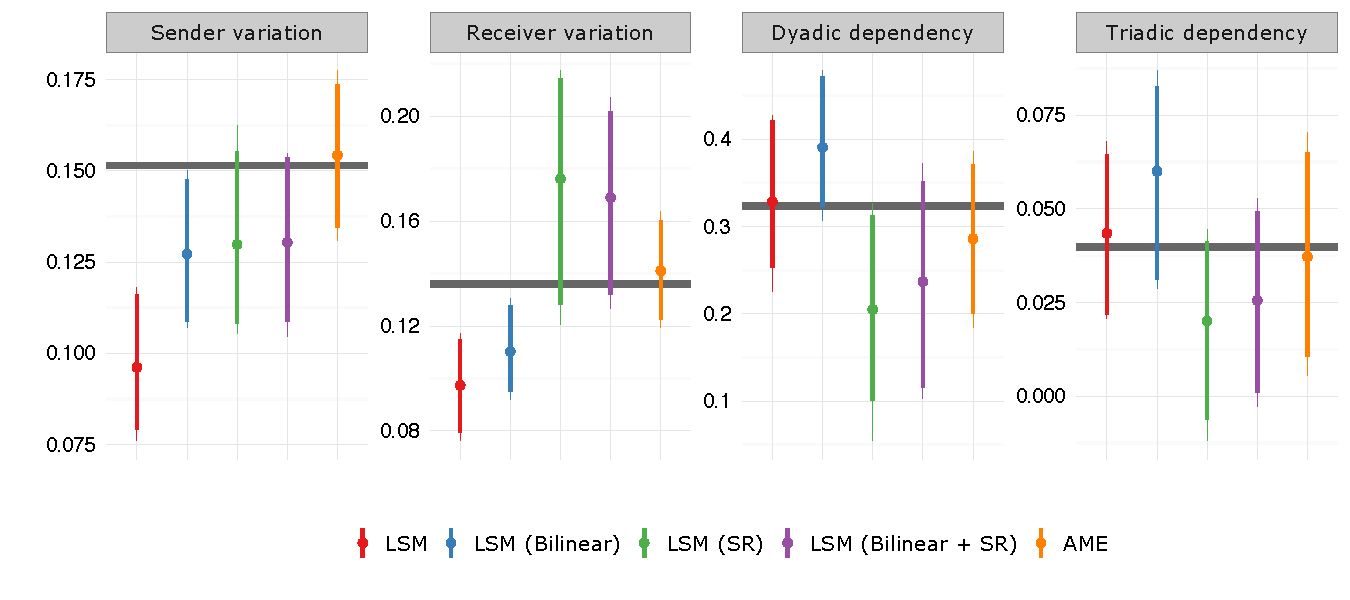
\includegraphics[width=1\textwidth]{netPerfCoef_latSpace}
	\caption{Posterior predictive goodness of fit summary}
	\label{fig:netPerfCoef_latSpace}
\end{figure}

\begin{figure}[ht]
	\centering
	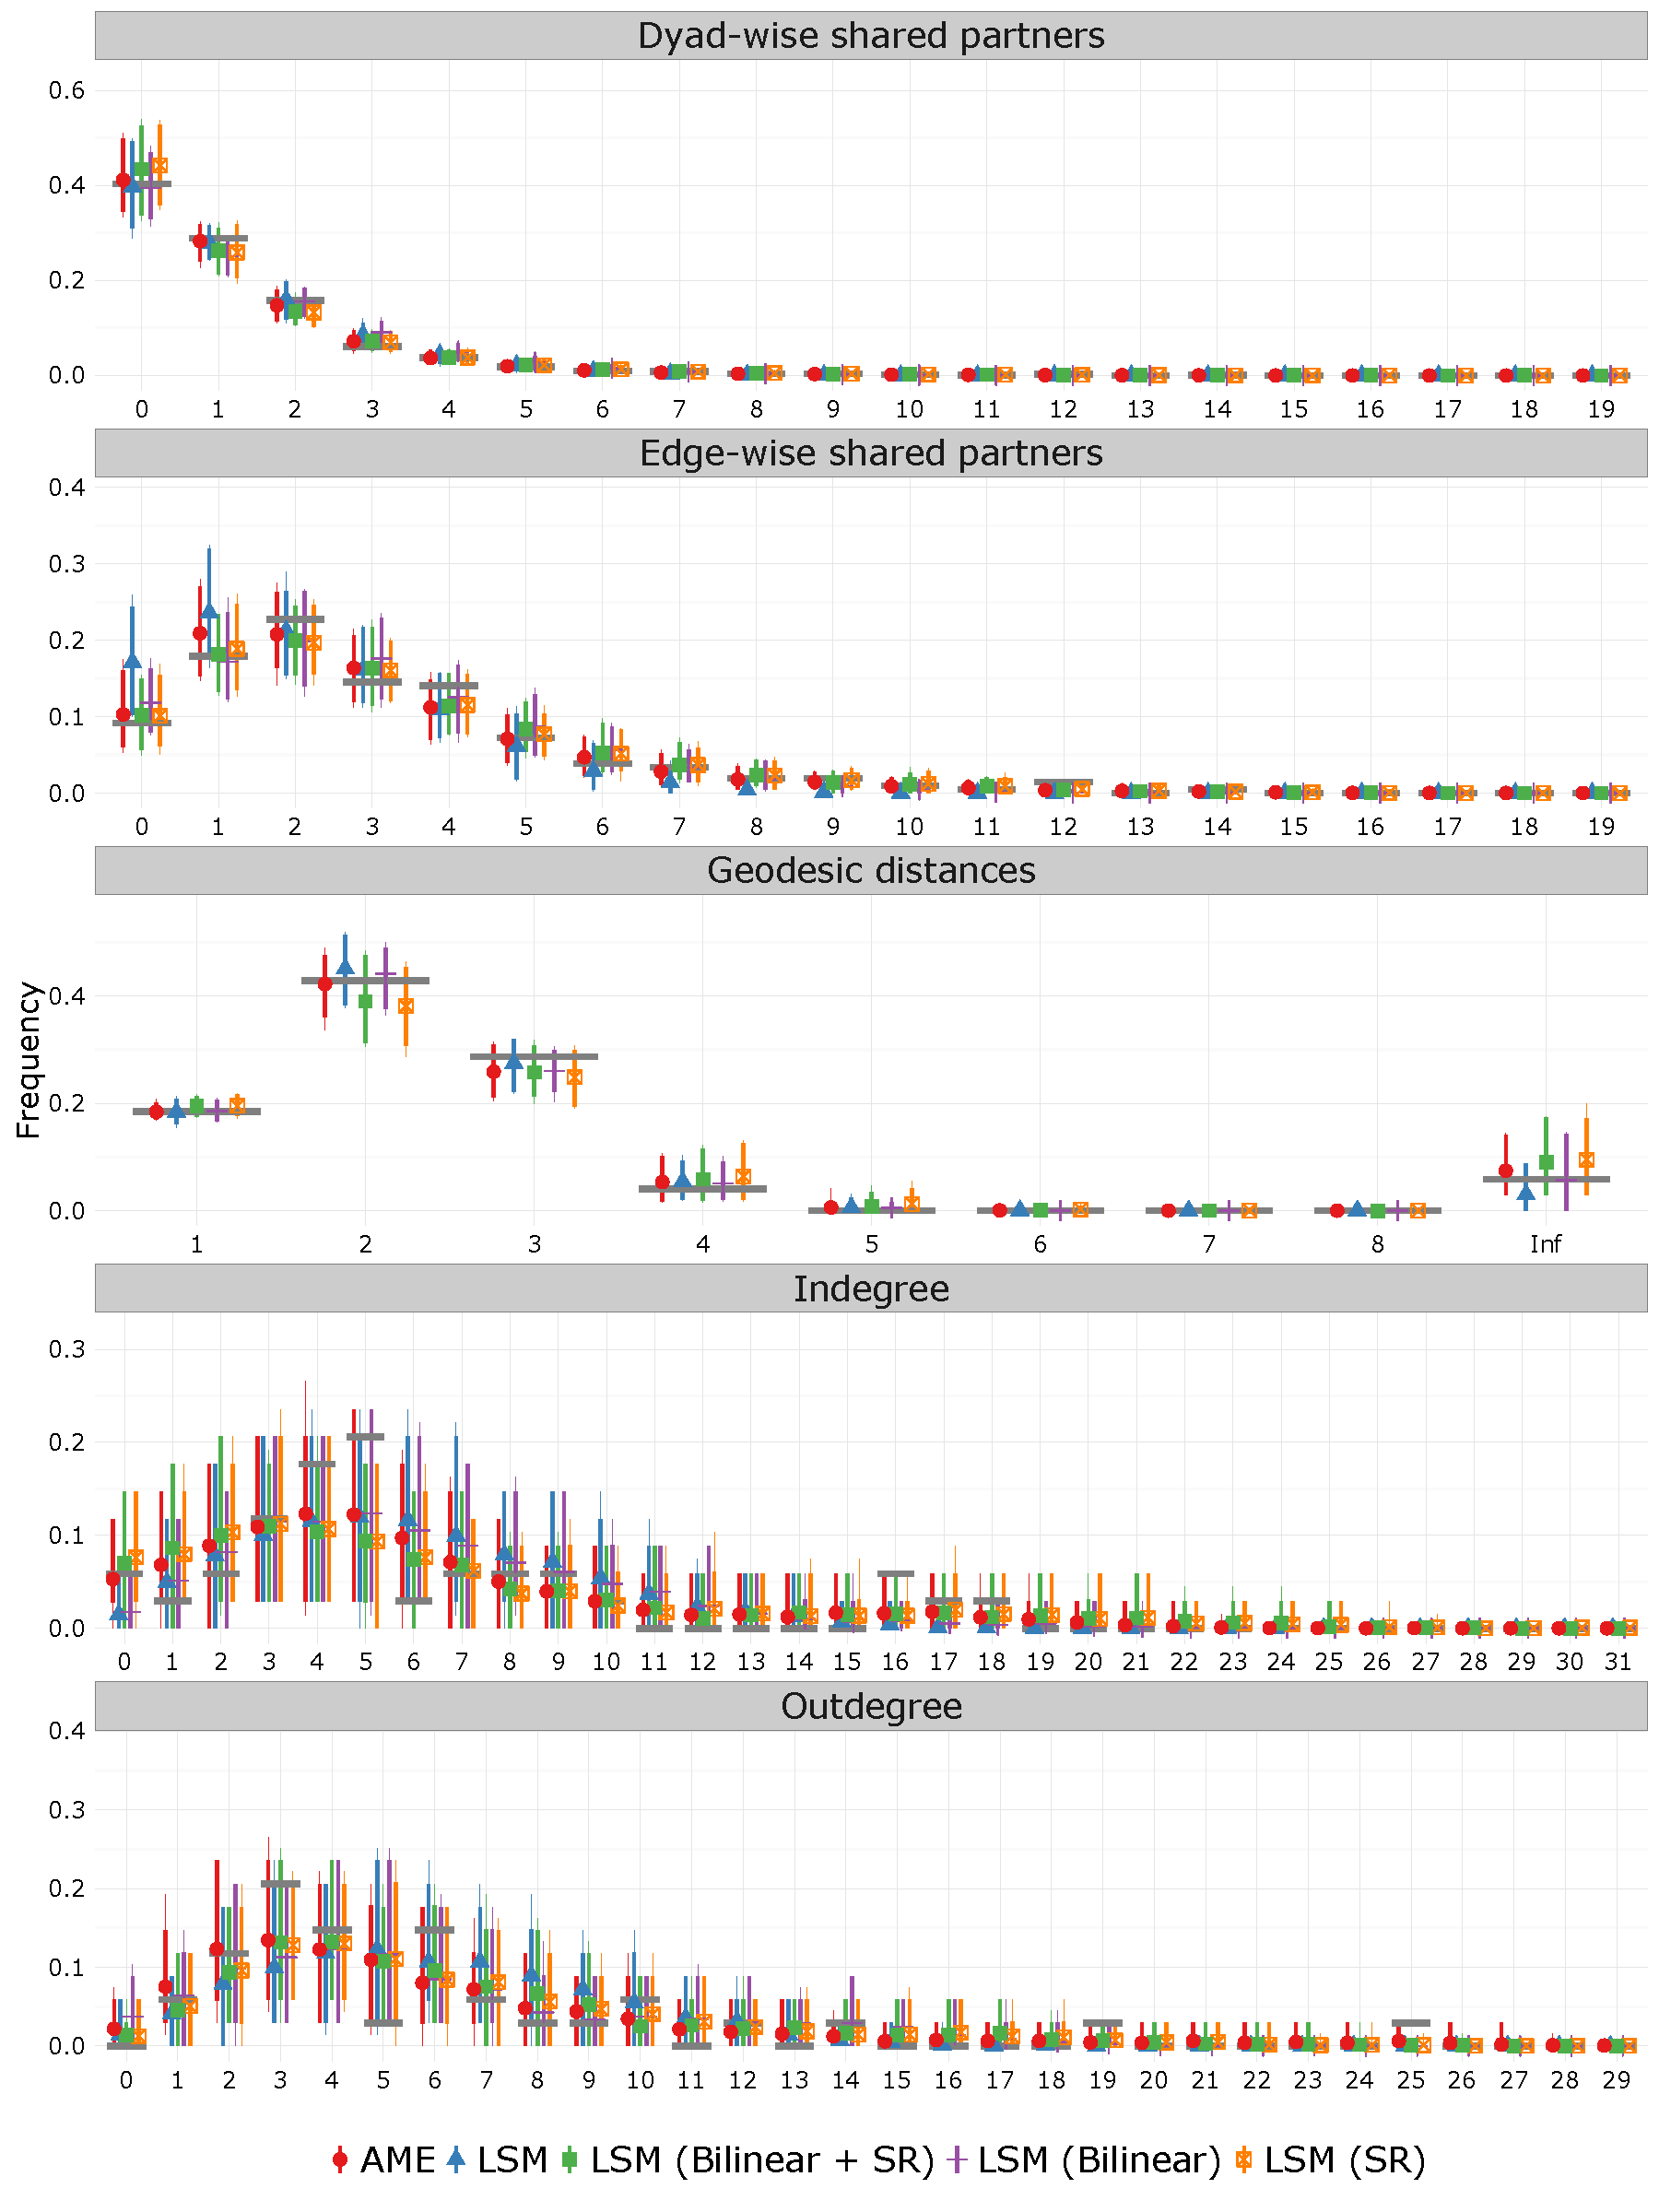
\includegraphics[width=1\textwidth]{ggGofAll_latSpace}
	\caption{network stats }
	\label{fig:gofAll_latSpace}
\end{figure}
\FloatBarrier
\newpage

\subsection{Comparison with other AME Parameterizations}

Here we provide a comparison of the AMEN model we presented in the paper that uses $K=2$ for multiplicative effects and show how results change when we use $K=/{1,3,4/}$. 

% latex table generated in R 3.5.0 by xtable 1.8-2 package
% Wed Jul 11 18:23:00 2018
\begin{table}[ht]
\centering
\begingroup\tiny
\begin{tabular}{lcccc}
   & AME (k=1) & AME (k=2) & AME (k=3) & AME (k=4) \\ 
  \hline
\hline
Intercept/Edges & -3.07 & -3.40 & -3.91 & -4.13 \\ 
   & [-3.87; -2.29] & [-4.40; -2.51] & [-5.90; -2.82] & [-5.93; -3.00] \\ 
  \textbf{Conflicting policy preferences} &  &  &  &  \\ 
  $\;\;\;\;$ Business vs. NGO & -1.27 & -1.38 & -1.52 & -1.54 \\ 
   & [-2.19; -0.47] & [-2.47; -0.49] & [-2.67; -0.53] & [-2.59; -0.47] \\ 
  $\;\;\;\;$ Opposition/alliance & 0.94 & 1.08 & 1.27 & 1.38 \\ 
   & [0.66; 1.27] & [0.72; 1.49] & [0.82; 2.10] & [0.87; 2.24] \\ 
  $\;\;\;\;$ Preference dissimilarity & -0.65 & -0.79 & -0.90 & -0.94 \\ 
   & [-1.28; -0.04] & [-1.55; -0.07] & [-1.78; -0.13] & [-1.77; -0.08] \\ 
  \textbf{Transaction costs} &  &  &  &  \\ 
  $\;\;\;\;$ Joint forum participation & 0.84 & 0.92 & 1.08 & 1.22 \\ 
   & [0.38; 1.31] & [0.40; 1.46] & [0.41; 1.96] & [0.50; 2.24] \\ 
  \textbf{Influence} &  &  &  &  \\ 
  $\;\;\;\;$ Influence attribution & 1.00 & 1.10 & 1.30 & 1.39 \\ 
   & [0.65; 1.40] & [0.70; 1.55] & [0.76; 2.29] & [0.82; 2.27] \\ 
  $\;\;\;\;$ Alter's influence indegree & 0.10 & 0.11 & 0.13 & 0.14 \\ 
   & [0.07; 0.13] & [0.07; 0.15] & [0.09; 0.20] & [0.09; 0.21] \\ 
  $\;\;\;\;$ Influence absolute diff. & -0.06 & -0.07 & -0.08 & -0.09 \\ 
   & [-0.09; -0.03] & [-0.11; -0.03] & [-0.15; -0.04] & [-0.16; -0.04] \\ 
  $\;\;\;\;$ Alter = Government actor & 0.52 & 0.56 & 0.65 & 0.72 \\ 
   & [0.00; 1.08] & [-0.06; 1.16] & [-0.05; 1.49] & [-0.01; 1.48] \\ 
  \textbf{Functional requirements} &  &  &  &  \\ 
  $\;\;\;\;$ Ego = Environmental NGO & 0.62 & 0.68 & 0.84 & 0.86 \\ 
   & [-0.28; 1.53] & [-0.36; 1.73] & [-0.43; 2.40] & [-0.49; 2.32] \\ 
  $\;\;\;\;$ Same actor type & 0.98 & 1.03 & 1.17 & 1.23 \\ 
   & [0.60; 1.37] & [0.62; 1.48] & [0.69; 1.83] & [0.70; 1.96] \\ 
   \hline
\hline
\end{tabular}
\endgroup
\caption{* p $<$ 0.05 (or 0 outside the 95\% confidence interval).} 
\label{tab:regTable_latSpace}
\end{table}


\begin{figure}[ht]
	\centering
	\begin{tabular}{cc}
	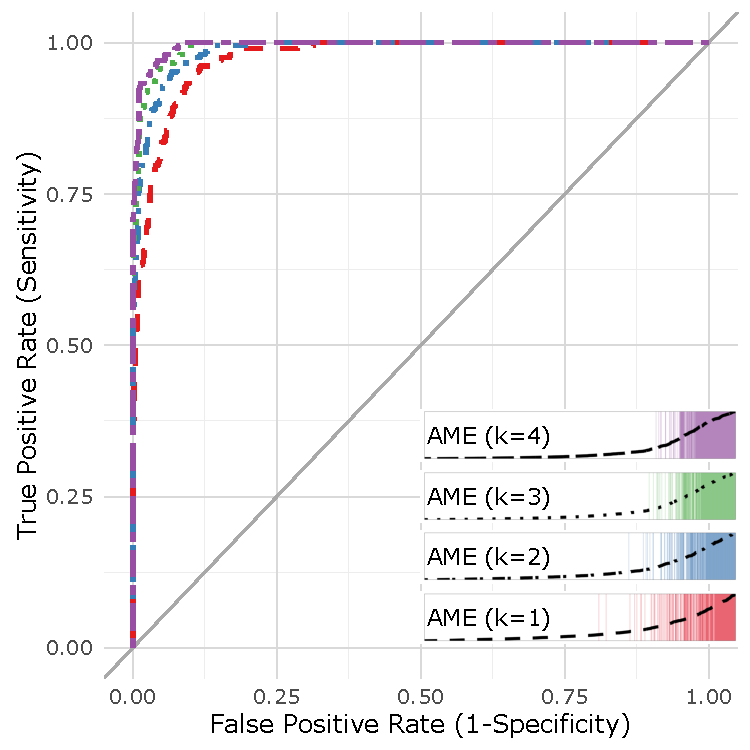
\includegraphics[width=.5\textwidth]{roc_ameSR} & 
	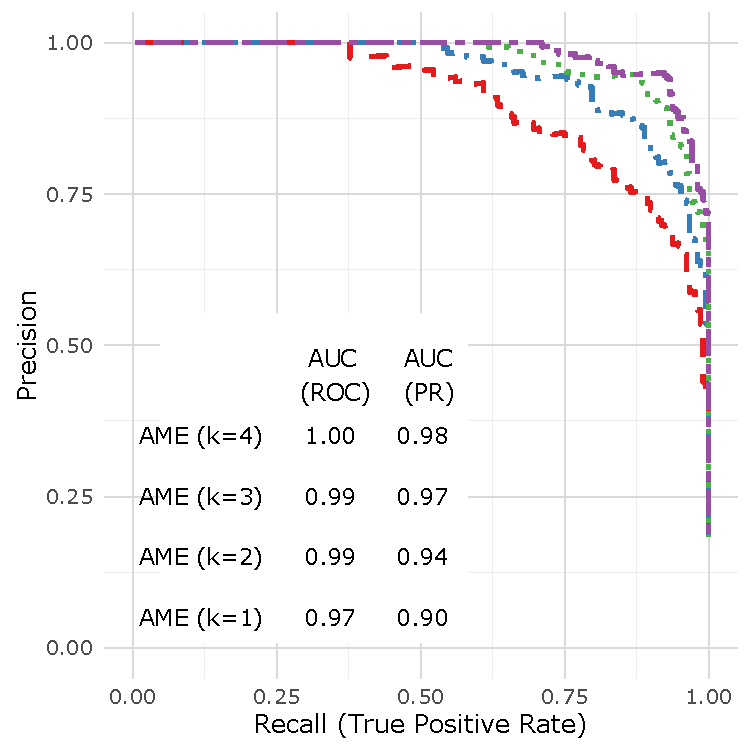
\includegraphics[width=.5\textwidth]{rocPr_ameSR}
	\end{tabular}
	\caption{ROC and separation plots}
	\label{fig:roc_latentSpace}
\end{figure}

\begin{figure}[ht]
	\centering
	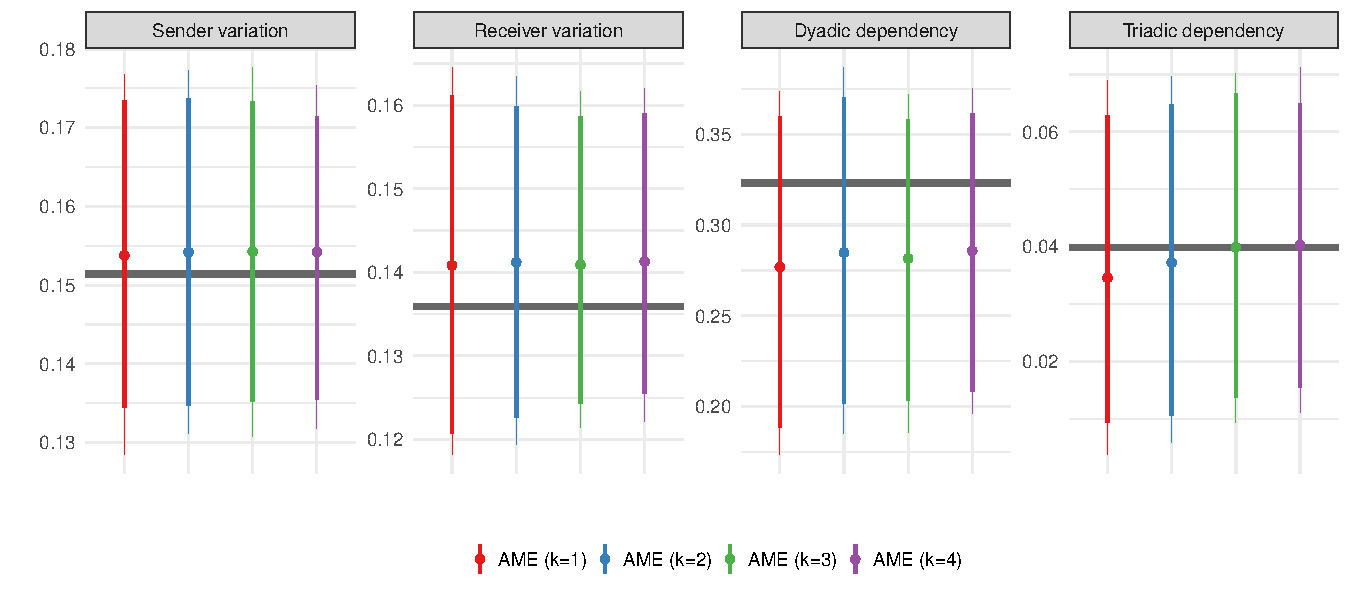
\includegraphics[width=1\textwidth]{netPerfCoef_ameSR}
	\caption{Posterior predictive goodness of fit summary}
	\label{fig:netPerfCoef_ameSR}
\end{figure}

\begin{figure}[ht]
	\centering
	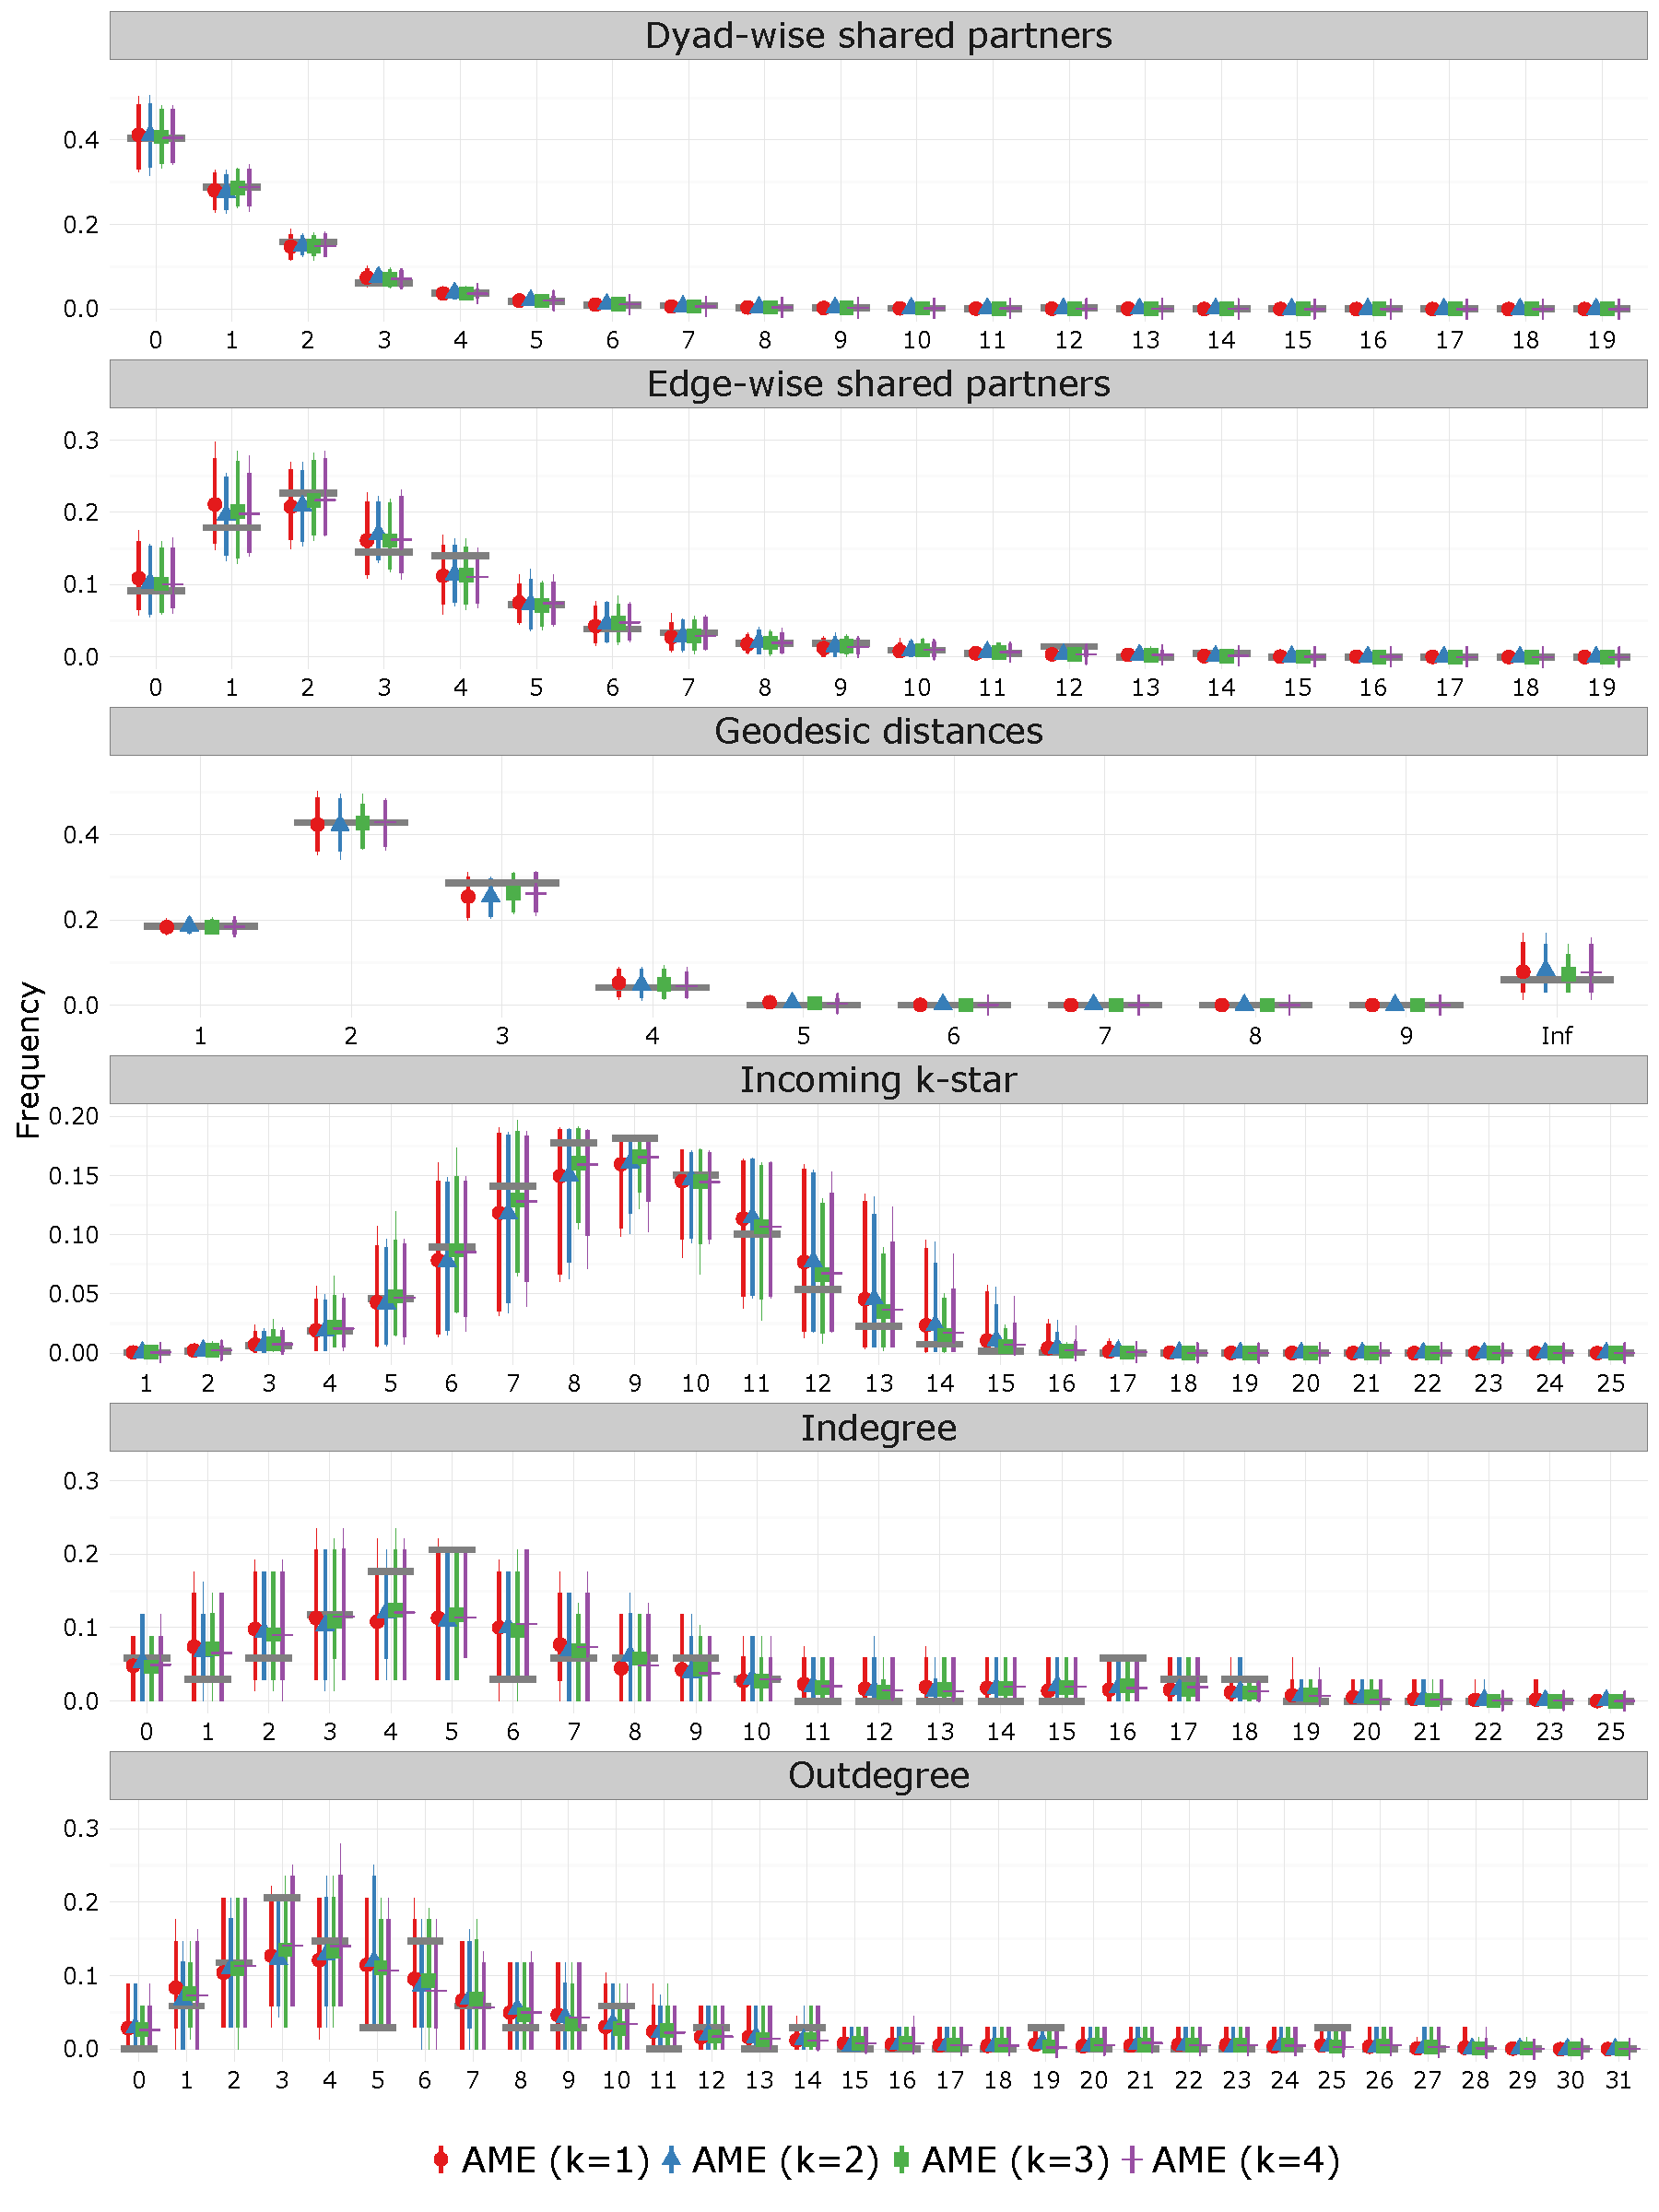
\includegraphics[width=1\textwidth]{ggGofAll_ameSR}
	\caption{network stats }
	\label{fig:gofAll_ameSR}
\end{figure}
\FloatBarrier

\newpage
\begin{figure}[ht]
	\centering
	\begin{tabular}{cc}
	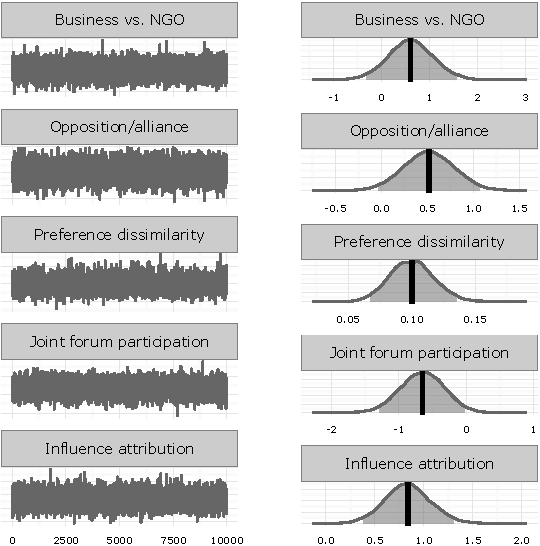
\includegraphics[width=.45\textwidth]{ameConv1_SR1} &
	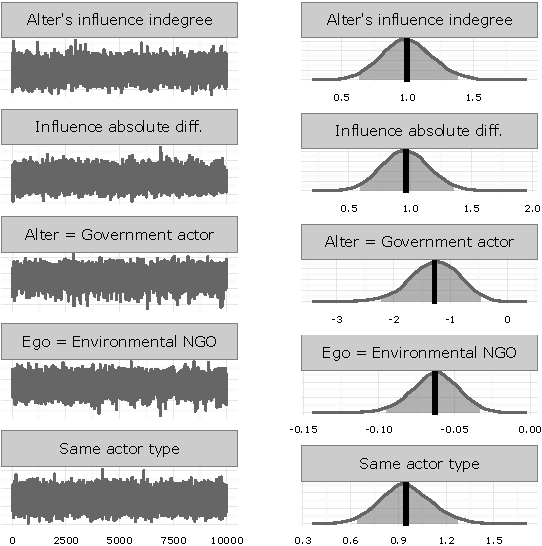
\includegraphics[width=.45\textwidth]{ameConv2_SR1}
	\end{tabular}
	\caption{MCMC chain for AMEN model in which we utilize the SRM to account for first and second-order dependence. To account for third order dependencies we use the latent factor approach discussed earlier with $K=1$.}
	\label{fig:ameConv}
\end{figure}

\begin{figure}[ht]
	\centering
	\begin{tabular}{cc}
	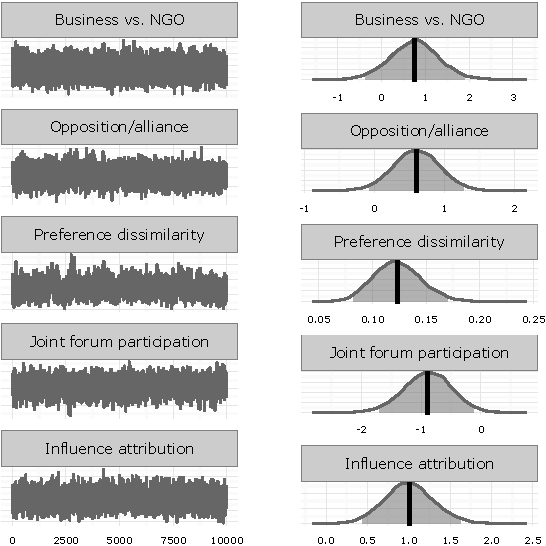
\includegraphics[width=.45\textwidth]{ameConv1_SR3} &
	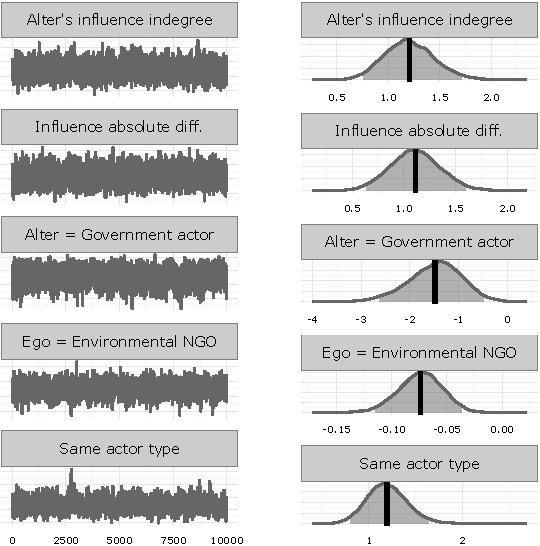
\includegraphics[width=.45\textwidth]{ameConv2_SR3}
	\end{tabular}
	\caption{MCMC chain for AMEN model in which we utilize the SRM to account for first and second-order dependence. To account for third order dependencies we use the latent factor approach discussed earlier with $K=3$.}
	\label{fig:ameConv}
\end{figure}
\FloatBarrier

\begin{figure}[ht]
	\centering
	\begin{tabular}{cc}
	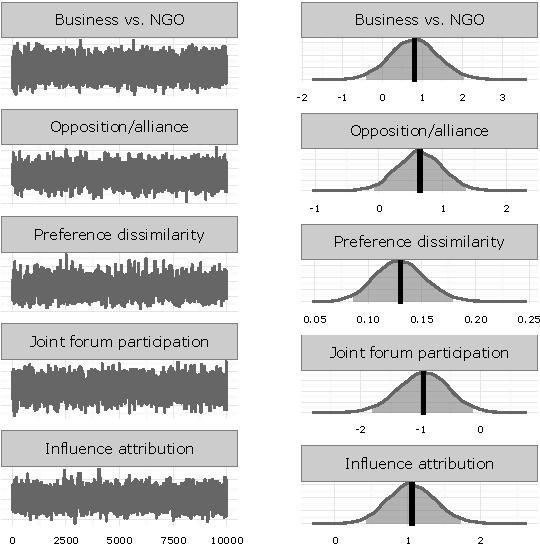
\includegraphics[width=.45\textwidth]{ameConv1_SR4} &
	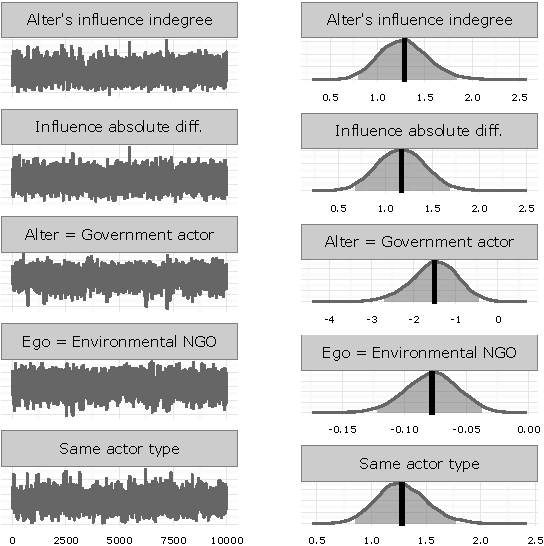
\includegraphics[width=.45\textwidth]{ameConv2_SR4}
	\end{tabular}
	\caption{MCMC chain for AMEN model in which we utilize the SRM to account for first and second-order dependence. To account for third order dependencies we use the latent factor approach discussed earlier with $K=4$.}
	\label{fig:ameConv}
\end{figure}
